\chapter{Experimentele analyse}\label{Experiment}

In hoofdstuk \ref{Lectuur} hebben we deze bouwstenen meer in detail bekeken om nu tot de experimentele analyse te komen. Voor de voorstelling van de dataset hebben we de Vector Space Methode gekozen (zie \ref{Voorstelling dataset}) . Nu in sectie \ref{De Dataset} gaan we dieper in op het verzamelen van de data voor deze experimentele analyse. Uiteindelijk is het beschikken over een goede dataset even belangrijk als het beschikken over goede technieken en evengoed een onderdeel van de experimentele analyse.\\
Deze analyse is opgedeeld in verschillende subanalyses om zo een optimaal beeld te krijgen over al dan niet de verschillen tussen Nederlandse en Engelse Gevoelsanalyse. 

Voor de gevoelsanalyse gebruiken we de voorverwerkingstechnieken uit sectie \ref{Technieken voor Pre-Processing} zoals het verwijderen van stopwoorden, Term weigthing en LSA. Ook gebruiken we de Naive Bayes Classifier en Decision tree uit sectie \ref{Leermethode} als leermethoden en proberen we een onderscheid te maken tussen recensies met een negatieve of positieve opinie. De prestaties van de gevoelsanalyses beoordelen we in dit onderzoek op basis van de precisie waarmee negatieve en positieve recensies worden onderscheiden.\\

Als eerste analyse beginnen we in \ref{Engelse gevoelsanalyse versus Nederlandse Gevoelsanalyse} met de verschillen te bekijken tussen Engelse en Nederlandse gevoelsanalyse op basis van de prestatie. Nadat we deze analyse hebben uitgevoerd, bekijken we in sectie \ref{Classificatie op basis van geannoteerde woordenlijsten} gevoelsanalyse met een andere eenvoudige en initu\"itievere kijk en analyseren we de classificatie op basis van geannoteerde woordenlijsten met gevoelens.

Afhankelijk van het positief karakter van de voorgaande analyses gaan we nog iets dieper in op het Nederlands in sectie \ref{Onderwerpgevoeligheid van Nederlandse Gevoelsanalyse} en analyseren we de onderwerp-gevoeligheid van Nederlandse gevoelsanalyse.

\section{De Dataset}\label{De Dataset}

Het verzamelen van data lijkt misschien een triviaal onderdeel van heel de experimentele analyse, maar dit is zeker niet het geval. Er moet heel verstandig en kritisch omgegaan worden bij het verzamelen van data voor gevoelsanalyse. Een eerste punt is sarcasme. Sarcasme is vandaag de dag nog altijd een onopgelost probleem (\cite{liebrecht2013perfect}) en is iets waar we rekening mee moeten houden als we de bron voor de verzameling van onze data selecteren. Sociale media zoals Twitter en dergelijke kunnen we dus voor onze gevoelsanalyse niet gebruiken. Een andere probleem is het labelen van de data, omdat we voor deze experimentele analyse supervised learning technieken gebruiken, is het heel arbeidsintensief om de data manueel te labelen.Echter Reviewsites bieden hier de oplossing. Deze sites laten gebruikers toe om omtrend een bepaald product een recensie te posten en hierbij ook een score mee te geven. Door die score kunnen we tijdens het verzamelen van de data, de recensies ook automatisch labelen.\\

Uiteraard zijn er enorm veel reviewsites beschikbaar en stuiten we hier op enkele problemen. Men moet rekening houden met het aanbod. Om een zo goed mogelijk beeld te krijgen willen we in onze datasets een algemeen onderwerp inbrengen. Dit wil zeggen dat we niet in het wilde weg recensies kunnen scrapen van iedere reviewsite dat we tegenkomen, maar selectief te werk moeten gaan. Als eerste ingeving gingen we de oplossing zoeken bij webshops zoals Coolblue \url{http://www.coolblue.be/}, Tweakers \url{http://tweakers.net/} en Amazon \url{http://www.amazon.com/}. Op deze website kan men een enorme hoeveelheid aan productrecensies, ideaal dus voor onze gevoelsanalyse. Het probleem echter bij deze websites is dat de reviews vaak te specifiek zijn en mogelijks de analyses kunnen be\"invloeden, door bijvoorbeeld een bepaald model van beamer meteen als doorweegfactor voor een positieve recensie te beschouwen.

\begin{figure}%
    \centering
    \subfloat{{
\includegraphics[width=15cm]{coolbuetweakers} }}%
    \caption{Enkele voorbeelden van reviews met verschillende onderwerpen, afkomstig van \url{http://www.coolblue.be} en \url{http://www.tweakers.net} }%
\end{figure}

Uiteindelijk hebben we de oplossing gevonden bij film-, muziek- en boekrecensies. Er al veel onderzoek gedaan naar Engelse gevoelsanalyse en filmrecensies zijn hier een populaire dataset. Dit maakt het voor ons mogelijk om Engelse datasets over te nemen uit eerder onderzoek. De Engelse dataset die we gebruiken in dit onderzoek is afkomstig uit een eerder onderzoek door \cite{maas-EtAl:2011:ACL-HLT2011}. Al deze gebruikersrecensies zijn toen gescraped geweest van de website imdb (\url{http://www.imdb.com/}) en zijn dus filmrecensies.\\
Voor de Nederlandse gevoelsanalyse waren er geen datasets beschikbaar en moeten we deze scrapen. De websites \url{moviemeter.nl}, \url{boekmeter.nl} en \url{muziekmeter.nl} vormen de perfecte bron aan informatie om te scrapen. Ze bevatten allemaal toplijsten met films, boeken of muziekalbums waarop in grote aantallen gebruikers hun persoonlijke mening plaatsen.\\

Belangrijk om te vermelden is dat zowel bij het labelen van de Engelse als de Nederlandse dataset dezelfde voorwaarden werd gerespecteerd. Enkel hoog gepolariseerde recensies worden beschouwd in de dataset. Onderzoek rond polarisatie classificatie (\cite{maas-EtAl:2011:ACL-HLT2011}) ondersteund deze keuze. Een recensie wordt negatief gelabeld als het een score heeft van 4 op 10 of minder. Een positieve labeling wordt gegeven aan recensies met een score van 6 op 10 of meer.\\

Later in \ref{Engelse gevoelsanalyse versus Nederlandse Gevoelsanalyse} gaan we de grenskeuze  nog beter analyseren, door de prestaties te vergelijken, wanneer er een hogere polarisatie wordt doorgevoerd.

\begin{figure}[h]%
    \centering
    \subfloat{{
\includegraphics[width=10cm]{voorbeeldrecensie} }}%
    \caption{Een voorbeeld van een positieve commentaar op \url{moviemeter.nl}}%
\end{figure}
\newline

Alle Nederlandse recensies zijn afkomstig van de ``All Time Top 250''-toplijst op de betreffende website.

\begin{figure}%
    \centering
    \subfloat{{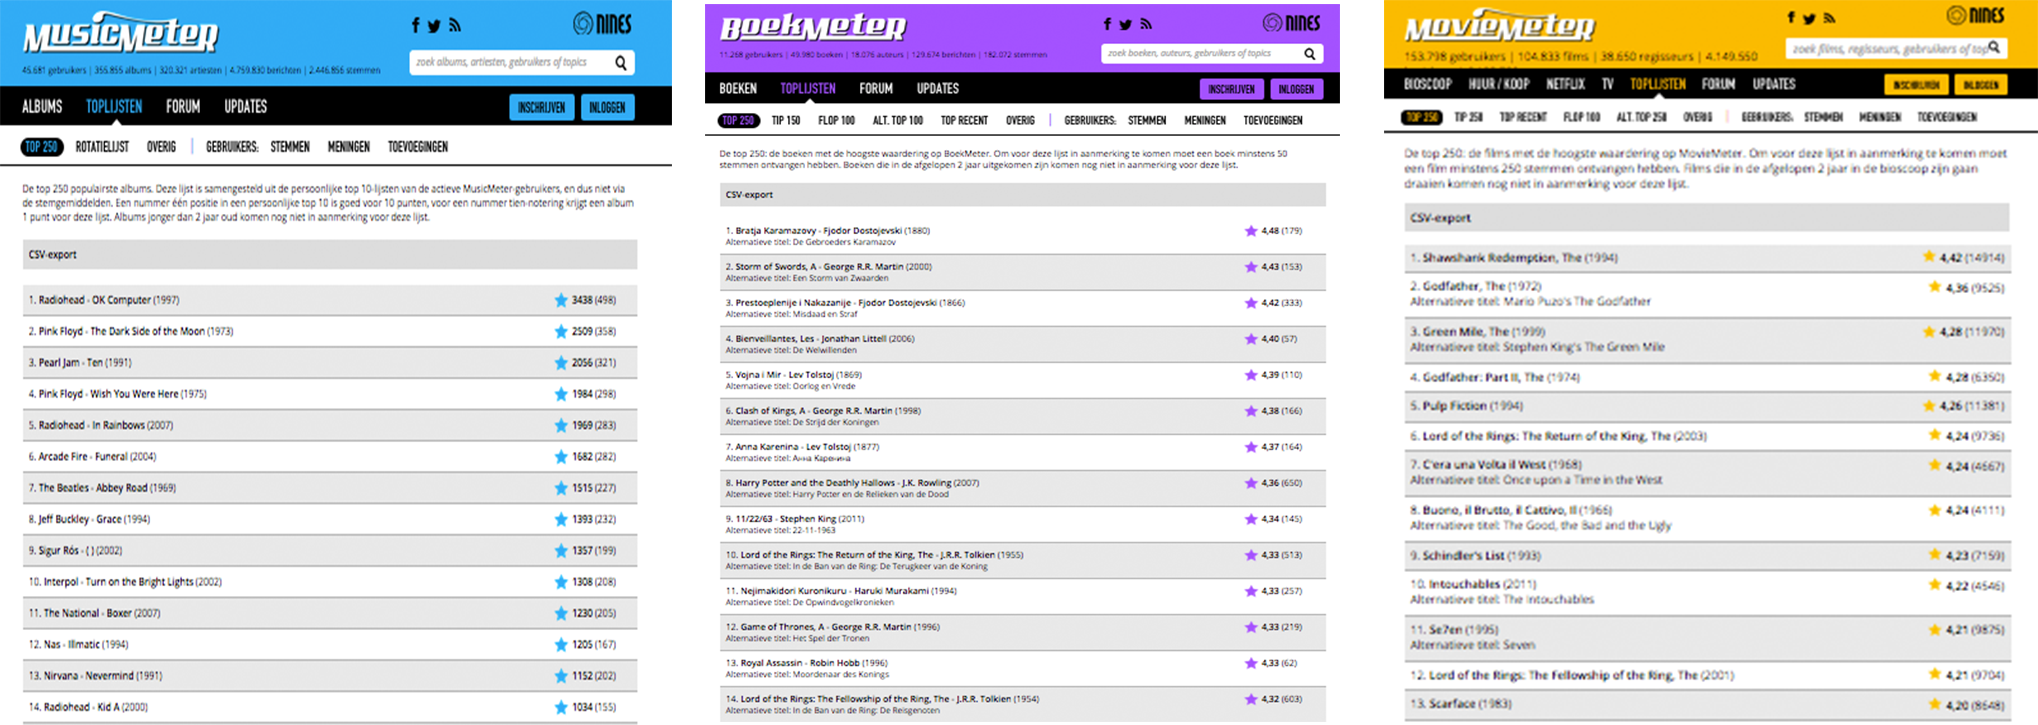
\includegraphics[width=15cm]{toplijsten} }}%
    \caption{de ``All Time Top 250''-toplijsten op de websites}%
\end{figure}

Onderstaande linkertabel geeft het aantal verzamelde Nederlandse recensies van ieder onderwerp weer, waarbij een onderscheid wordt gemaakt tussen positief en negatief. Analoog wordt dit in de rechtertabel voor de Engelse recensies weergegeven.\\

\begin{table}[h]
\centering
\setlength\tabcolsep{2pt}
\begin{minipage}[t]{0.48\textwidth}
\centering
\begin{tabular}{l|l|l|}
\cline{2-3}
                                      & Positief & Negatief \\ \hline
\multicolumn{1}{|l|}{Filmrecensies}   & 197358   & 17978    \\ \hline
\multicolumn{1}{|l|}{Muziekrecensies} & 15197    & 3019     \\ \hline
\multicolumn{1}{|l|}{Boekrecensies}   & 146      & 3719     \\ \hline
\end{tabular}
\caption{Aantal verzamelde Nederlandse recensies} 
\label{tabel: aantal verzamelde Nederlandse recensies}
\end{minipage}%
\hfill
\begin{minipage}[t]{0.48\textwidth}
\centering
\begin{tabular}{l|l|l|}
\cline{2-3}
                            & Positief & Negatief \\ \hline
\multicolumn{1}{|l|}{Films} & 197358   & 17978    \\ \hline
\end{tabular}
\caption{Aantal verzamelde Engelse recensies}
\end{minipage}
\end{table}

Wat meteen opvalt is dat het aantal verzamelde positieve boekrecensies heel klein is tegen over de andere recensies. Later bij het gebruik van deze dataset in \ref{Onderwerpgevoeligheid van Nederlandse Gevoelsanalyse} zullen we hier rekening mee moeten houden.\\

Om nog een beter inzicht te krijgen over de dataset geven onderstaande tabellen nog wat extra statistieken weer over de datasets.\\

\begin{table}[h]
\centering
\setlength\tabcolsep{2pt}
\begin{minipage}[t]{0.48\textwidth}
\centering

\begin{tabular}{l|l|l|}
\cline{2-3}
                & Positief & negatief \\ \hline
\multicolumn{1}{|l|}{Filmrecensies}   & 60       & 75       \\ \hline
\multicolumn{1}{|l|}{Muziekrecensies} & 89       & 105      \\ \hline
\multicolumn{1}{|l|}{Boekrecensies}   & 58       & 61    \\ \hline   
\end{tabular}

\caption{Gemiddeld aantal woorden voor een Nederlandse recensie} 
\label{tabel: Gemiddeld aantal woorden per recensie Nederlands}
\end{minipage}%
\hfill
\begin{minipage}[t]{0.48\textwidth}
\centering

\begin{tabular}{l|l|l|}
\cline{2-3}
                                   & Positief & Negatief \\ \hline
\multicolumn{1}{|l|}{Filmrecensie} & 229      & 228      \\ \hline
\end{tabular}
\caption{Gemiddeld aantal woorden voor een Engelse recensie}
\label{tabel: Gemiddeld aantal woorden per recensie Engels}
\end{minipage}
\end{table} 

Uit de tabel kunnen we afleiden dat de verzamelde Engelse filmrecensies gemiddeld veel langer zijn. De mogelijke invloed op de prestatie van dit gegeven, onderzoeken we verder in \ref{Engelse gevoelsanalyse versus Nederlandse Gevoelsanalyse}.

\begin{table}[h]
\centering
\setlength\tabcolsep{2pt}
\begin{minipage}[t]{0.48\textwidth}
\centering
\begin{tabular}{l|l|l|}
\cline{2-3}
                                      & Positief & Negatief \\ \hline
\multicolumn{1}{|l|}{Filmrecensies}   & 2,64\%   & 7,41\%   \\ \hline
\multicolumn{1}{|l|}{Muziekrecensies} & 7,44\%   & 12,52\%  \\ \hline
\multicolumn{1}{|l|}{Boekrecensies}   & 10,29\%  & 25,39\%  \\ \hline
\end{tabular}

\caption{Percentage woorden van het totaal aantal woorden in de Nederlandse dataset dat uniek is.} 
\end{minipage}%
\hfill
\begin{minipage}[t]{0.48\textwidth}
\centering
\begin{tabular}{l|l|l|}
\cline{2-3}
                                    & Positief & Negatief \\ \hline
\multicolumn{1}{|l|}{Filmrecensies} & 4,39\%   & 4,41\%   \\ \hline
\end{tabular}
\caption{Percentage woorden van het totaal aantal woorden in de Engelse dataset dat uniek is.} 
\end{minipage}
\end{table}


In \ref{Engelse gevoelsanalyse versus Nederlandse Gevoelsanalyse} voeren we ook een analyse uit zonder gebruik te maken van een dataset om uit te leren, maar classificeren we de gegeven recensies op basis geannoteerde woordenlijsten van gevoelens.  
Als bron voor deze woordenlijsten hebben we het \textit{Opinion lexicon} gebruikt, dat voor het eerst werd samengesteld door \cite{hu2004mining}. Deze woordenlijsten bestaan uit een lijst met negatieve en een lijst met positieve woorden. De lijsten bevatten in totaal ongeveer 6800 woorden en zijn enkel in het Engels verkrijgbaar. De Nederlandse woordenlijsten hebben we verkregen door de Engelse lijsten te vertalen met behulp van Google vertalen.\\

Onderstaande tabel geeft weer hoe de woordenlijsten zich tegenover elkaar verhouden.

\begin{table}[h]
\centering
\caption{Aantal woorden in iedere woordenlijst}
\label{table: Verlies in woordenschat}
\begin{tabular}{l|l|l|}
\cline{2-3}
 & Positief & Negatief \\ \hline
\multicolumn{1}{|l|}{Engels Woordenlijsten}     & 2006     & 4783     \\ \hline
\multicolumn{1}{|l|}{Nederlands Woordenlijsten} & 2006     & 4647     \\ \hline
\end{tabular}
\end{table}

We zien dat er een klein verlies van woorden is bij de negatieve Nederlandse woordenlijst. Dit komt door de vertaling van het Engels naar het Nederlands.

\begin{figure}%
    \centering
    \subfloat{{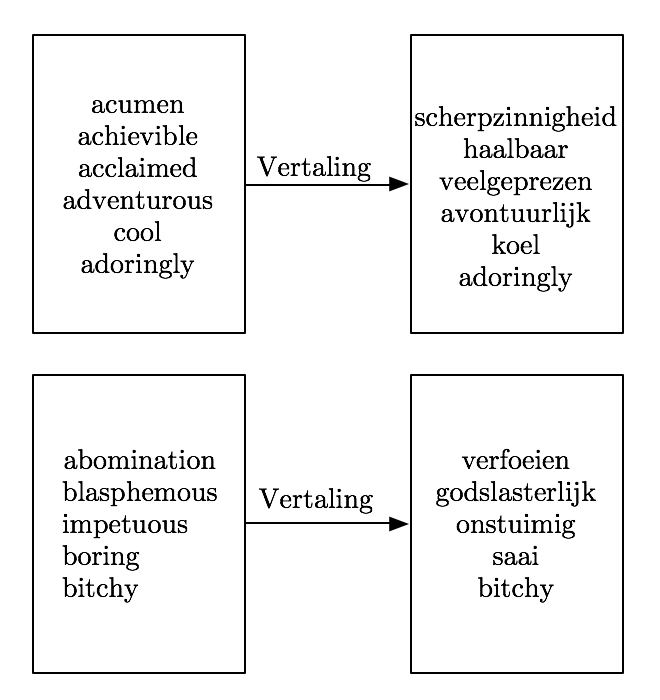
\includegraphics[width=7cm]{vbwoordenlijsten} }}%
    \caption{enkele voorbeelden uit de woordenlijsten. Links bevinden zich positieve en negatieve woorden uit de Engelse woordenlijsten, rechts bevinden zich de vertalingen naar het Nederlands.}
\end{figure}

\section{Engelse gevoelsanalyse versus Nederlandse Gevoelsanalyse}\label{Engelse gevoelsanalyse versus Nederlandse Gevoelsanalyse}

Als eerste analyse vergelijken we de Engelse gevoelsanalyse met de Nederlandse gevoelsanalyse. Als datasets gebruiken we de Nederlandse en Engelse filmrecensies, besproken in sectie \ref{De Dataset}. De filmrecensies stellen we voor aan de hand van de Vector Space Methode uit \ref{Vector Space Methode}, waarbij iedere filmrecensie wordt voorgesteld als een vector met zijn woordfrequenties. Als Classifiers gebruiken we de Naive Bayes Classifier en de Decision Tree, beide werden besproken in sectie \ref{Leermethode}. Bij de analyse vergelijken we ook alle voorverwerkingstechnieken uit \ref{Technieken voor Pre-Processing} en zelf combinaties hier van. Deze analyse is zodanig opgesteld dat we al de resultaten van de verschillende classifiers met een specifieke voorverwerkingstechniek naast elkaar kunnen leggen en de prestaties kunnen vergelijken voor wanneer men een Engelse of Nederlandse dataset gebruikt.\\

Concreter is de gevoelsanalyse die we in dit onderzoek uitvoeren, het correct kunnen onderscheiden van positieve en negatieve filmrecensies. De vergelijking wordt dan telkens gemaakt op basis van de prestaties van de analyses. De prestatie wordt beoordeeld op basis van de precisie waarmee de classifier de recensies classificeert. De precisie die we opnemen in onze resultaten voor een classifier wordt bepaald door het gemiddelde te nemen van 30 runs. Bij iedere run wordt er een ongetrainde classifier getraind met een trainingsset en wordt de precisie getest door het classificeren van de testset. In dit experiment bestaat iedere trainingsset uit 6000 filmrecensies en testset uit 2000 filmrecensies. Ook zorgen we er telkens voor dat zowel de trainingsset als de testset willekeurig en gebalanceerd samengesteld worden. Dit wil zeggen dat de datasets telkens voor de helft uit positieve en de andere helft uit negatieve recensies bestaan en wanneer men deze willekeurig zou classificeren, men een precisie baseline van $50\%$ krijgt.\\

Zoals eerder vermeld gebruiken we voor onze analyse de verschillende voorverwerkingstechnieken uit \ref{Technieken voor Pre-Processing}. We hebben ook de vrijheid genomen om verschillende voorverwerkingstechnieken te combineren en hier de resultaten van te bekijken.\\
Onderstaande tabellen geeft de belangrijkste resultaten weer van de gevoelsanalyses. In bijlage A vindt men de volledig tabel met de resultaten. \\ 
Bag of words (zie rij 1) gebruiken we in deze tabel als baseline om de invloed van de andere technieken te vergelijken. Om een overzicht te krijgen hebben we in de tabellen de resultaten die beter presteren dan Bag of Word vet gedrukt. 

\begin{table}[h]
\centering
\begin{adjustbox}{width=1\textwidth}
\begin{tabular}{|l|l|l|l|}
\hline
{\bf Nr} & \{\bf Title\}                                                                       & \{\bf Precisie Naive Bayes Classifier\} & \{\bf Precisie Decision Tree\} \\ \hline
1        & Bag of Words                                                                        & 85,74\%                                 & 69,06\%                        \\ \hline
2        & Best Feature selection on Bag of Words (max features)                               & 67,79\%                                 & {\bf 69,43\%}                  \\ \hline
3        & Best Feature selection on TFIDF (max features)                                      & 74,90\%                                 & {\bf 69,79\%}                  \\ \hline
4        & Bigram Collocaties                                                                  & {\bf 89,23\%}                           & {\bf 69,41\%}                  \\ \hline
5        & LSA on Bag of Words (max features)                                                  & 63,11\%                                 & 62,07\%                        \\ \hline
6        & LSA on TFIDF (max features)                                                         & 78,98\%                                 & {\bf 71,54\%}                  \\ \hline
7        & Term Weighting                                                                      & {\bf 86,75\%}                           & {\bf 69,76\%}                  \\ \hline
8        & Term Weighting + Bigrams                                                            & {\bf 89,00\%}                           & {\bf 69,28\%}                  \\ \hline
9        & Verwijderen van stopwoorden                                                         & {\bf 86,62\%}                           & {\bf 69,45\%}                  \\ \hline
10        & Verwijderen van stopwoorden + Best feature selection on Bag of Words (max features) & 74,43\%                                 & {\bf 69,36\%}                  \\ \hline
11       & Verwijderen van stopwoorden + Best feature selection on TFIDF (max features)        & 74,94\%                                 & {\bf 69,47\%}                  \\ \hline
12       & Verwijderen van stopwoorden + Bigram Collocaties                                    & {\bf 89,23\%}                           & {\bf 69,51\%}                  \\ \hline
13       & Verwijderen van stopwoorden + Bigram Collocaties + Term Weighting                   & {\bf 89,29\%}                           & {\bf 69,44\%}                  \\ \hline
14       & Verwijderen van stopwoorden + LSA on Bag of Words (max features)                    & 54,88\%                                 & 68,66\%                        \\ \hline
15       & Verwijderen van stopwoorden + LSA on TFIDF (max features)                           & 73,58\%                                 & {\bf 75,50\%}                  \\ \hline
16       & Verwijderen van stopwoorden + Term Weighting                                        & {\bf 87,41\%}                           & {\bf 69,60\%}                  \\ \hline
\end{tabular}
\end{adjustbox}

\caption{Resultaten experiment op Engelse recensies}
\label{tabel: resultaten engelse gevoelsanalyse}
\end{table}

\begin{table}[h]
\centering
\begin{adjustbox}{width=1\textwidth}
\begin{tabular}{|l|l|l|l|}
\hline
{\bf Nr} & {\bf \{\bf Title\}}                                                                  & \{\bf Precisie Naive Bayes Classifier\} & \{\bf Precisie Decision Tree\} \\ \hline
1        & Bag of Words                                                                         & 70,51\%                                 & 59,34\%                        \\ \hline
2        & Best Feature selection Bag of Words                                                  & 58,86\%                                 & {\bf 59,45\%}                  \\ \hline
3        & Best Feature selection on TFIDF ( max features)                                      & 59,53\%                                 & {\bf 59,35\%}                  \\ \hline
4        & Bigram Collocaties                                                                   & 70,20\%                                 & {\bf 59,35\%}                  \\ \hline
5        & LSA on Bag of Words                                                                  & 54,84\%                                 & 57,53\%                        \\ \hline
6        & LSA on TFIDF (100 features)                                                          & 63,15\%                                 & 58,58\%                        \\ \hline
7        & Term Weighting                                                                       & 69,40\%                                 & 58,83\%                        \\ \hline
8        & Term Weighting + Bigrams                                                             & 67,96\%                                 & 59,06\%                        \\ \hline
9        & Verwijderen van stopwoorden                                                          & 70,35\%                                 & 56,82\%                        \\ \hline
10        & Verwijderen van stopwoorden + Best feature selection on Bag of Words ( max features) & 60,76\%                                 & 56,74\%                        \\ \hline
11       & Verwijderen van stopwoorden + Best feature selection on TFIDF (max features)         & 59,18\%                                 & 56,44\%                        \\ \hline
12       & Verwijderen van stopwoorden + Bigram Collocaties                                     & {\bf 70,63\%}                           & 56,80\%                        \\ \hline
13       & Verwijderen van stopwoorden + Bigram Collocaties + Term Weighting                    & {\bf 70,66\%}                           & 56,58\%                        \\ \hline
14       & Verwijderen van stopwoorden + LSA on Bag of Words (100 features)                     & 53,74\%                                 & 57,23\%                        \\ \hline
15       & Verwijderen van stopwoorden + LSA on TFIDF (max features)                            & 60,15\%                                 & 59,24\%                        \\ \hline
16       & Verwijderen van stopwoorden + Term Weighting                                         & {\bf 70,54\%}                           & 56,55\%                        \\ \hline
\end{tabular}
\end{adjustbox}

\caption{Resultaten experiment op Nederlandse recensies}
\label{tabel: resultaten Nederlandse gevoelsanalyse}
\end{table}


Wat meteen opvalt als we de resultaten bekijken in tabel \ref{tabel: resultaten engelse gevoelsanalyse} en \ref{tabel: resultaten Nederlandse gevoelsanalyse} is het algemeen beter presteren van de technieken op de Engelse dataset. Tabel \ref{tabel: verschil engels en nederlandse prestatie} geeft het verschil in prestatie aan tussen het Engels en het Nederlands. We zien dat de prestatie op de Engelse dataset gemiddeld 13\% beter presteert bij de Naive Bayes Classifier en 10\% beter bij de Decision Tree.


\begin{table}[h]
\centering
\begin{adjustbox}{width=1\textwidth}
\begin{tabular}{|l|l|l|}
\hline
{\bf Title}                                                                          & {\bf Verschil in Precisie Naive Bayes Classifier} & {\bf Verschil in Precisie Decision Tree} \\ \hline
Bag of Words                                                                         & 14,72\%                                           & 16,05\%                                  \\ \hline
Best Feature selection Bag of Words                                                  & 8,78\%                                            & 12,18\%                                  \\ \hline
Best Feature selection on TFIDF ( max features)                                      & 15,36\%                                           & 10,44\%                                  \\ \hline
Bigram Collocaties                                                                   & 16,25\%                                           & 10,41\%                                  \\ \hline
LSA on Bag of Words                                                                  & 27,27\%                                           & 10,37\%                                  \\ \hline
LSA on TFIDF (100 features)                                                          & 19,83\%                                           & 10,69\%                                  \\ \hline
Term Weighting                                                                       & 11,79\%                                           & 10,89\%                                  \\ \hline
Term Weighting + Bigrams                                                             & 21,04\%                                           & 10,22\%                                  \\ \hline
Verwijderen van stopwoorden                                                          & 31,79\%                                           & 11,92\%                                  \\ \hline
Verwijderen van stopwoorden + Best feature selection on Bag of Words ( max features) & 35,55\%                                           & 12,22\%                                  \\ \hline
Verwijderen van stopwoorden + Best feature selection on TFIDF (max features)         & -2,56\%                                           & 12,61\%                                  \\ \hline
Verwijderen van stopwoorden + Bigram Collocaties                                     & 18,60\%                                           & 12,61\%                                  \\ \hline
Verwijderen van stopwoorden + Bigram Collocaties + Term Weighting                    & 13,67\%                                           & 12,61\%                                  \\ \hline
Verwijderen van stopwoorden + LSA on Bag of Words (100 features)                     & 15,09\%                                           & 12,48\%                                  \\ \hline
Verwijderen van stopwoorden + LSA on TFIDF (max features)                            & -15,67\%                                          & 12,11\%                                  \\ \hline
Verwijderen van stopwoorden + Term Weighting                                         & 3,93\%                                            & 5,63\%                                   \\ \hline
{\bf Gemiddeld verschil}                                                             & {\bf 13,40\%}                                     & {\bf 10,83\%}                            \\ \hline
\end{tabular}
\end{adjustbox}
\caption{Verschil in precisie tussen het Engelse en het Nederlands (Eng - NL)}
\label{tabel: verschil engels en nederlandse prestatie}
\end{table}

Nu in tabel \ref{tabel: Gemiddeld aantal woorden per recensie Engels} uit \ref{De Dataset} zien we dat de Engelse dataset gemiddeld meer woorden heeft dan de Nederlandse dataset. Dit kan mogelijks een positieve invloed hebben op de classificatie, aangezien hoe meer woorden, hoe meer informatie betekent voor de classifier en het zo beter kan classificeren. Om dergelijke stelling te kunnen onderbouwen voeren we een kleine extra analyse uit. We voeren opnieuw een gevoelsanalyse uit op beide datasets, enkel beperken we het aantal woorden per recensie voor zowel de Engelse als de Nederlandse dataset tot de eerste 60 woorden. Als referentie gebruiken we de best presterende combinatie van voorverwerkingstechniek en classifier. Dit is de Naive Bayes Classifier met als voorverwerkingstechniek \textit{Verwijderen van stopwoorden + Bigram Collocaties + Term Weighting} (zie rij 13).

\begin{table}[h]
\centering
\begin{tabular}{l|l|}
\cline{2-2}
                                                  & {\bf Precisie Testset} \\ \hline
\multicolumn{1}{|l|}{{\bf Engelse recensies}}     & 82,21\%                \\ \hline
\multicolumn{1}{|l|}{{\bf Nederlandse recensies}} & 69,96\%                \\ \hline
\end{tabular}
\caption{classificatieprecisie van Naive Bayes Classifier met Verwijderen van stopwoorden + Bigrams + Term Weighting, waarbij iedere recensie werd beperkt tot de eerste 60 woorden}
\end{table}

Ook is het interessant om te zien naar het verschil in de prestatie van de classifiers voor een bepaalde voorverwerkingstechniek. Bij rij 13 in tabel \ref{tabel: resultaten engelse gevoelsanalyse} zien we bijvoorbeeld een verschil van bijna 20 \%. Na een kleine subanalyse waarbij we kijken naar de recensies waarbij de ene classifier de recensie juist classificeert en de andere fout, zien we dat....\\

\begin{table}[h]
\centering
\caption{My caption}
\label{my-label}
\begin{tabu}{|p{\myWidth}|l|l|l|}  %to \textwidth %{|p{\myWidth}|X|X|X|}
\hline
 & {\bf NB heeft} & {\bf DT heeft} & {\bf Opinie} \\ \hline
Best een goede thriller.Maar echt super vind ik hem niet.Vond hem soms te langdradig en saai. & Positief & Negatief & Positief \\ \hline
Onvoorstelbaar dat deze in de top 250 staat. Het is geen verhaal, geen begin, geen einde, geen doel, echt waardeloos. 0,5 ster voor Sandra Bullocks. & Negatief & Positief & Negatief \\ \hline
Naar mijn smaak te veel een bewegende graphic novel.Aan de ene kant is het indrukwekkend hoe dit wordt vormgegeven (kleurgebruik, shots), aan de andere kant voegt het medium film naar mijn idee weinig toe aan het verhaal.Ik kreeg tijdens het kijken als het ware het gevoel een graphic novel te lezen ipv een film te kijken. Het visuele aspect overheerste naar mijn idee teveel.Dit is dan ook de reden dat ik op een lage score uitkom: 2* voor verbluffend vormgegeven bewegende stripplaatjes. & Negatief & Positief & Negatief \\ \hline
\end{tabu}
\end{table}

Verder zien we ook dat de prestatie voor beide talen een grotere spreiding heeft bij de Naive Bayes Classifier dan bij de Decision tree. Voor het Engels vallen de resultaten van de Naive Bayes Classifier binnen een interval van 36\% en bij de Decision Tree heeft dit interval een lengte van 14\%. Voor het Nederlandse we hetzelfde verschijnsel. De resultaten van de Naive Bayes classifier vallen binnen een interval van 18\% en bij de Decision tree is dit 2\%. Dit valt terug te koppelen naar de theorie. De Naive Bayes Classifier baseert zich op basis van probabiliteit. Hier zit veel meer vrijheid in en kan beter om met afwijkingen. Waarbij we dit met de Decision tree niet hebben. Er wordt een beslissingsboom opgesteld op basis van de trainingsset en het is dan veel moeilijk om iets ongezien, wat helemaal niet het deductief patroon volgt, te classificeren.

Dan als er naar de prestaties van de voorverwerkingtechnieken per classifier kijken. We nemen zoals eerder vermeld in \ref{Bag of Words} nemen we Bag of Words (zie rij 1) als referentie om de prestatie van de andere technieken te vergelijken.\\
Als we nu kijken naar de Naive Bayes Classifier komen de pre-processing technieken: Bigram collocaties, Term Weighting en het verwijderen van stopwoorden positief naar voren. Alleen of in combinatie hebben ze een positieve invloed op de prestatie. Dit is het geval voor beide talen, al is deze bevinding bij het Engels overtuigend aanwezig en bij het Nederlands eerder minimaal. Opmerkelijk is dat de combinatie van de drie pre-processing technieken bij beide talen als best presterende techniek naar boven komt. Opnieuw is bij het Nederlands dit verschil minimaal ten op zichten van de andere combinaties.\\
Voor de Decision tree springt de prestatie van \textit{Verwijderen van stopwoorden + LSA + Term weighting} in het oog met 75\%als beste resultaat. Bij het Nederlands springt deze techniek er niet uit en is de prestatie zelfs minder goed als Bag of Words, al is het verschil miniem en hoort het nog steeds bij de betere resultaten van de Decision Tree.\\

Voor het verwijderen van stopwoorden zagen we in tabel \ref{tabel: verschil in verwijderde stopwoorden} dat het verschil tussen het aantal originele features en het aantal aangepast features eerder klein is en het totale aantal nog niet reduceert met 0,5\%. Echter bij het Engels zien we een kleine verbetering bij de Naive Bayes Classifier door het verwijderen van stopwoorden (zie rij 9). Bij het Nederlands is dit niet zo zichtbaar. Maar wat we wel zien is dat bijna alle technieken samen met de Naive Bayes Classifier een positieve invloed hebben op de prestatie als ze in combinatie zijn met het verwijderen van stopwoorden. Merk op dat die combinatie altijd in combinatie is met Bigrams of  Term weighting. Om hier duidelijkheid in te krijgen voeren we hier nog een kleine subanalyse uit, die de permutaties van deze technieken gaat bekijken.

Resultaten hier + bla bla


Een punt van kritiek dat we gaven in sectie \ref{De Dataset} bij het verzamelen van de dataset is de drempel wanneer de recensie als positief of al negatief wordt beschouwd. Bovenstaande resultaten zijn allemaal bereikt door de drempel voor een positieve recensie op een score van 6 op 10 of meer te zetten en voor en negatieve recensie deze op 4 op 10 of minder te zetten.
Nu eerder was aangetoond dat de polarisatie van de dataset een rol speelt bij de classificatie (\cite{maas-EtAl:2011:ACL-HLT2011}). Daarom voeren nog een subanalyse uit met de best presterende techniek namelijk de techniek op rij 13 met de Naive Bayes Classifier en bekijken we hoe de polarisatie van de dataset de prestatie van de classifier be\"invloed. De trainingsset bestaat telkens uit 6000 filmrecensies en de testset uit 2000 filmrecensies.


\begin{table}[h]
\centering
\caption{Prestaties bij een hogere polariteit. Telkens wordt de kritische score voor een positieve en negatieve recensie in de eerste kolom gegeven door pos - neg  }
\begin{tabular}{l|l|}
\cline{2-2}
                          & Precisie \\ \hline
\multicolumn{1}{|l|}{6-3} & 70,40\%  \\ \hline
\multicolumn{1}{|l|}{7-3} & 76,02\%  \\ \hline
\multicolumn{1}{|l|}{8-2} & 77,83\%  \\ \hline
\multicolumn{1}{|l|}{9-1} & 79,61\%  \\ \hline
\end{tabular}
\end{table}


Algemeen kunnen we zeggen dat de trends die we zien bij het Engels zich ook voordoen bij het Nederlands. De technieken werken ook op het Nederlands, als men weet dat in eerder onderzoek \cite{pang2002thumbs} aantoont dat een human-based classifier resultaten haalt van ongeveer 58\% tot 64\% op Engelse filmreviews, kunnen we stellen dat de technieken goede prestaties halen op Nederlandse reviews, met als de Naive Bayes Classifier de best presterende van de twee leermethoden.


\section{Classificatie op basis van geannoteerde woordenlijsten}\label{Classificatie op basis van geannoteerde woordenlijsten}

Om meer inzicht te krijgen over de verschillen in de gevoelsanalyse bij de twee talen, voeren we nog een tweede analyse uit. Bij dit experiment gaan we heel eenvoudig en intu\"itief te werk. We kijken hoe de classificatie verloopt, wanneer we enkel geannoteerde woordenlijsten met gevoelens in beschouwing nemen. Er wordt voor iedere recensie bekeken, hoeveel woorden van de recensie voorkomen in de positieve lijst en hoeveel in de negatieve. De lijst met de meest overeenkomstige woorden geeft aan of de recensie positief of negatief moet worden geclassificeerd.\\
Voor de woordenlijsten gebruiken we de eerder vermeldden woordenlijsten uit \ref{De Dataset}. De classificatie zelf testen we op de Engelse en Nederlandse filmrecensies.\\
Onderstaande tabel geeft de resultaten van de classificatie weer met als precisie het gemiddelde van 30 runs en een testset van 2000 samples random en gebalanceerd samengesteld. Merk op dat de classifier kan ook onbeslist blijven over een recensie wanneer het totaal aantal voorkomens in de positieve woordenlijst even groot is als het aantal voorkomens in de negatieve woordenlijst.Voor deze analyse beschouwen we een onbesliste recensie meteen als fout geclassificeerd.

\begin{table}[h]
\centering
\begin{tabular}{l|l|}
\cline{2-2}
                                           & Precisie \\ \hline
\multicolumn{1}{|l|}{Engels recensies}     & 67,43\%  \\ \hline
\multicolumn{1}{|l|}{Nederlands recensies} & 36,82\%   \\ \hline
\end{tabular}
\caption{Classificatieprecisie aan de hand van woordenlijsten}
\end{table}

 Het resultaat voor Engelse recensies met 68\% is goed, maar voor het Nederlands met 1\% kunnen we zeggen dat de classificatie methode niet werkt. Merk op dat onze dataset altijd gebalanceerd was en dus bij een randomclassificatie een baseline van 50\% haalt. Echter omdat we elke onbesliste recensie meteen als fout beschouwen, komen we aan een veel slechter percentage dan 50\%.\\
 Omwille van de slechte resultaten van het Nederlands, zijn we de woordenlijst iets meer in detail gaan bekijken. Een eerste bevinding is dat de leenwoorden niet correct worden omgezet door Google translate. De woorden uit de Engelse woordenlijst kunnen juist vertaald zijn door Google translate, maar kunnen onnatuurlijk overkomen in het Nederlands. Bijvoorbeeld het positieve woord \textit{cool} wordt vertaald door Google translate als \textit{koel}, wat in het Nederlands helemaal niet wordt gebruikt als positief woord.\\
 Het is daarom interessant om te kijken, wat de prestatie is voor het Nederlandse gevoelsanalyse wanneer men enkel de Engelse woordenlijst gebruikt. Of wanneer we de Engelse en Nederlandse woordenlijsten samenvoegen.

\begin{table}[h]
\centering
\begin{tabular}{l|l|l|l|l|}
\cline{2-5}
                                         & {\bf Precisie} & {\bf Positief} & {\bf Negatief} & {\bf Gemiddeld} \\ \hline
\multicolumn{1}{|l|}{{\bf Eng + Ned WL}} & 38,27\%        & 3,49           & 3,00           & 3,25            \\ \hline
\multicolumn{1}{|l|}{{\bf Eng WL}}       & 26,18\%        & 0,35           & 1,34           & 0,84            \\ \hline
\end{tabular}
\caption{My caption}
\end{table}

 Verder is de oorsprong van de woordenlijsten ook iets waar we rekening mee moeten houden . De woordenlijsten zijn samengesteld op basis van Engelse recensies en  het verlies in de vertaling naar het Nederlands kan een mogelijk effect hebben op de Nederlandse classficatie. Al zien we in tabel \ref{table: Verlies in woordenschat} dat dit verlies beperkt wordt tot 2,5\%. Ook is de gebruikte woordenschat in het Engels niet hetzelfde als in het Nederlands om zich positief uit te drukken. Om hier een volledig beeld over te krijgen, wat hier de invloed van is hebben we een kleine subanalyse uitgevoerd. Bij deze analyse zijn we gaan kijken hoe veel woorden er nu effectief uit de woordenlijst werden teruggevonden in de dataset met recensies.\\

\begin{table}[h]
\centering
\begin{tabular}{l|l|l|l|}
\cline{2-4}
                                                 & {\bf Positief} & {\bf Negatief} & {\bf Gemiddeld} \\ \hline
\multicolumn{1}{|l|}{{\bf Engelse woordenlijst}} & 6,32           & 6,32           & 6,32            \\ \hline
\multicolumn{1}{|l|}{{\bf Nederlands}}           & 3,40           & 1,79           & 2,59            \\ \hline
\end{tabular}
\caption{test test}
\end{table}

Als laatste moet en we ook opmerken dat internetslang, typefouten en uitgesmeerde woorden zoals \textit{sssaaaaiiii} niet in rekening worden gebracht bij woordenlijsten en is een probleem dat moeilijk te vermijden is. 

In verder onderzoek kan men een groot deel van de invloeden, zoals de verkeerde vertaling van leenwoorden of andere woordenschat vermijden door eigenhandig een Nederlandse geannoteerde woordenlijst met gevoelens samen te stellen op basis van filmrecensies. Mogelijks kan dit de prestatie verbeteren.


\section{Onderwerpgevoeligheid van Nederlandse Gevoelsanalyse}\label{Onderwerpgevoeligheid van Nederlandse Gevoelsanalyse}

Nu we weten welke methoden presteren op het Nederlands en welke niet, kunnen we ons nog iets specifieker toeleggen op taalvarianten binnen het Nederlands. De voorgaande analyses in \ref{Engelse gevoelsanalyse versus Nederlandse Gevoelsanalyse} en \ref{Classificatie op basis van geannoteerde woordenlijsten} zijn altijd uitgevoerd op filmrecensies en hadden goede prestaties. Het is interessant om te bekijken of er een onderwerpgevoeligheid is binnen het Nederlands. Voor een bepaald onderwerp kan men een bepaalde taal of jargon hebben. Het is daarom ook eens interessant dit te onderzoeken. \\

Concreet voor deze analyse gebruiken we enkel een van de beste presterende techniek uit \ref{Engelse gevoelsanalyse versus Nederlandse Gevoelsanalyse}, namelijk de Naive Bayes Classifier in combinatie met Term weighting en het verwijderen van stopwoorden. We kijken hoe deze techniek presteert wanneer we het trainen en testen met recensies over hetzelfde onderwerp en hoe het presteert met een verschillend onderwerp.  Als datasets nemen we film- , muziek en boekrecensies. De prestatie van de classifiers is telkens de gemiddelde classificatieprecisie van 30 runs, waarbij de trainingsset uit 6000 recensies bestaat en de testset uit 2000 recensies. Met uitzondering de boekrecensies, daarbij wordt de classifier telkens getraind met 266 boekrecensies en werd er getest met 144 boekrecensies. De reden is het extreem laag aantal aan verzamelde positieve boekrecensies (zie tabel \ref{tabel: aantal verzamelde Nederlandse recensies}).


Onderstaande kruistabel met classificatieprecisies vat de belangrijkste resultaten van het experiment samen. De volledige resultaten vindt men in bijlage B. Merk op dat men hier ook de controle op over- of onderfitting vindt. Over- en onderfitting zijn symptomen bij machine learning waarbij men de classifier over of ondertrained. Voor de volledigheid hebben we deze grafieken in de bijlage toegevoegd.    

\begin{table}[h]
\centering
\begin{tabular}{l|c|c|c|}
\cline{2-4}
                                      & \textbf{Films} & \textbf{Muziek} & \textbf{Boeken} \\ \hline
\multicolumn{1}{|l|}{\textbf{Films}} & 70,66\%         & 61,00\%         & 56,25\%         \\ \hline
\multicolumn{1}{|l|}{\textbf{Muziek}} & 62,07\%         & 82,62\%         & 56,47\%         \\ \hline
\multicolumn{1}{|l|}{\textbf{Boeken}} & 65,87\%         & 61,46\%         & 71,76\%         \\ \hline
\end{tabular}
\label{tab:alles}
\caption{Kruistabel van alle classificatieresultaten met de kolommen het onderwerp van de trainingsset en de rijen het onderwerp van de testset.} 
\end{table}

Als laatste hebben nog de confusion matrixen van het experiment. Een confusion matrix geeft weer hoeveel recensies er juist en fout geclassificeerd zijn. 

\begin{table}[h]
\centering
\setlength\tabcolsep{4pt}
\begin{minipage}[t]{0.48\textwidth}
\centering
\begin{tabular}{lll}
                                 & \textbf{P}               & \textbf{N}               \\ \cline{2-3} 
\multicolumn{1}{l|}{\textbf{P'}} & \multicolumn{1}{l|}{43\%} & \multicolumn{1}{l|}{6\%} \\ \cline{2-3} 
\multicolumn{1}{l|}{\textbf{N'}} & \multicolumn{1}{l|}{18\%} & \multicolumn{1}{l|}{31\%} \\ \cline{2-3} 
\end{tabular}
\caption{Gemiddelde confusion matrix in percent voor een Naive Bayes Classifier, waar trainings- en testset over hetzelfde onderwerp gaan}
\end{minipage}%
\hfill
\begin{minipage}[t]{0.48\textwidth}
\centering
\begin{tabular}{lll}
                                 & \textbf{P}               & \textbf{N}               \\ \cline{2-3} 
\multicolumn{1}{l|}{\textbf{P'}} & \multicolumn{1}{l|}{32\%} & \multicolumn{1}{l|}{18\%} \\ \cline{2-3} 
\multicolumn{1}{l|}{\textbf{N'}} & \multicolumn{1}{l|}{21\%} & \multicolumn{1}{l|}{29\%} \\ \cline{2-3} 
\end{tabular}
\caption{Gemiddelde confusion matrix in percent voor een Naive Bayes Classifier, waar trainings- en testset over een verschillend onderwerp gaan} 
\end{minipage}
\end{table}

\begin{table}[h!]
\centering
\begin{tabular}{c >{\bfseries}r @{\hspace{0.7em}}c @{\hspace{0.4em}}c @{\hspace{0.7em}}l}
  \multirow{10}{*}{\parbox{1.1cm}{\bfseries\raggedleft eigelijke\\ waarde}} & 
    & \multicolumn{2}{c}{\bfseries voorspelde waarde} & \\
  & & \bfseries p & \bfseries n  \\
  & p$'$ & \MyBox{Waar}{Positief} & \MyBox{Vals}{Negatief}  \\[2.4em]
  & n$'$ & \MyBox{Vals}{Positief} & \MyBox{Waar}{Negatief} \\
\end{tabular}
\caption{Illustratie van de confusion matrix} 
\end{table}


Op basis van de tabel kunnen we zeggen dat het trainen en testen met het zelfde onderwerp het beste resultaat geeft. We kunnen dit observatie terugkoppelen naar de theorie. Aangezien men de classifier traint op een bepaald onderwerp, krijgt de classifier een bepaalde idee over het concept. In dit geval bijvoorbeeld wat nu juist positieve en negatieve recensies zijn binnen filmrecensies. Wanneer de classifier als testset een dataset krijgt dat in lijn is met het aangeleerde concept gaat de precisie altijd hoger liggen dan wanneer de testset half of helemaal niet in lijn ligt met het aangeleerde concept. En dit is ook hier geval wanneer men een classifier traint op filmrecensies en test met filmrecensies of muziekrecensies. De precisie met als testset filmrecensies ligt hoger. Er is wel een overlap tussen de concepten, aangezien we nog degelijke resultaten hebben bijvoorbeeld bij het trainen op films en testen op muziek. Bij een getrainde classifier op boekrecenies is de prestatie minder met een vreemde testset. Merk op dat we in \ref{De Dataset} hadden vermeld dat het verzameld aantal positieve boekrecensies heel laag is  en dat dit mogelijke oorzaak kan zijn van de slechte prestatie. De dataset is groot genoeg om het concept over boekrecensies aan te leren, maar te klein om een overlappend concept aan te leren over wat in een algemeen een positieve en negatieve recensies is.

Verder springt de prestatie van wanneer men traint en test met muziekrecensies in het oog. Ten opzichte van de andere onderwerpen, waarbij trainingsset en testset met hetzelfde onderwerp werd gebruikt, is er een verschil van ongeveer 10\%. Een mogelijk oorzaak kan bij de lengte van de muziekrecensie liggen. Als we terugkijken naar tabel \ref{tabel: Gemiddeld aantal woorden per recensie Nederlands}, zien we dat de muziekrecensies gemiddeld langer zijn dan de andere recensies. Om dergelijke invloed te onderzoeken, voeren we een kleine subanalyse uit, waarbij we de lengte van de recensies beperken tot 63 woorden. 63 is de gemiddelde lengte van al de andere recensies. \\

\begin{table}[h]
\centering
\caption{My caption}
\label{my-label}
\begin{tabular}{l|l|}
\cline{2-2}
                                          & {\bf Precisie} \\ \hline
\multicolumn{1}{|l|}{{\bf Muziek (60 w)}} & 81,44\%        \\ \hline
\multicolumn{1}{|l|}{{\bf Muziek (10 w)}} & 74,53\%        \\ \hline
\end{tabular}
\end{table}

Voor beide matrixen, ziet men duidelijk dat positieve recensies beter ge\"identificeerd worden. Na het herbekijken van de datasets, waarbij we kijken naar de valse positieve zagen we dat....\\

Voorbeelden van vals positieve opzoeken.

Een mogelijk verklaring dat mensen zich bij een positieve recensie zich veel expressiever en uitgebreider uitdrukken dan bij een negatieve recensie. Hierdoor krijgt de classifier meer informatie over de features van een positief document waardoor het beter het concept ``Positief'' kan bepalen 


